\documentclass[tikz,border=5pt]{standalone}
\usepackage[T1]{fontenc}
\usepackage{lmodern,amsmath}
\usetikzlibrary{arrows.meta,calc}
\definecolor{ink}{HTML}{27374A}
\definecolor{llmfill}{HTML}{EEECFA}
\definecolor{llmline}{HTML}{7764AA}
\definecolor{statefill}{HTML}{E8F3F1}
\definecolor{stateline}{HTML}{408578}
\definecolor{execfill}{HTML}{FFF0DE}
\definecolor{execline}{HTML}{B97B35}
\definecolor{controlfill}{HTML}{F5F7FA}
\begin{document}
% Sources: Zheng et al. (2026), Sections 3.4 and 6; released implementation
% c4d52cf99bd870d830b456ac7c0684aec1aef375, agent.py/world_model.py/config.yaml.
% Diagram describes the baseline runtime, including the released execution gate.
% agent.py:119 search policy; 293/326/367 generation; 531 step; 634 execution gate.
% world_model.py:128 prompt; 455 tournament_rank; 653 should_execute.
% journal.py:201 get_best_node; 211 generate_summary. Report preparation: paper Sec. 3.4.
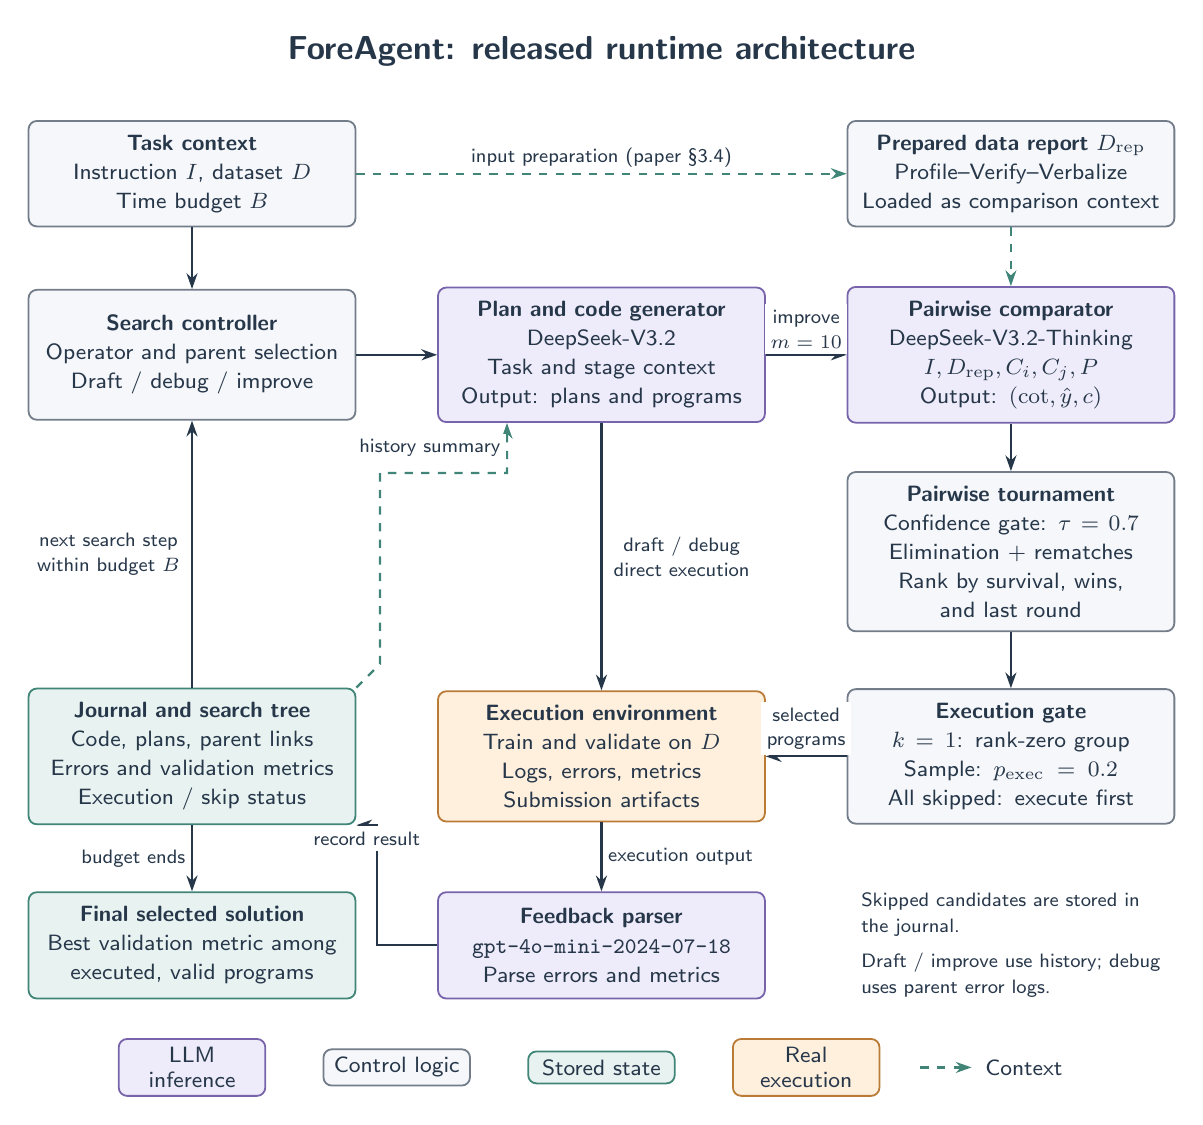
\begin{tikzpicture}[
  font=\sffamily\fontsize{8.5}{10.5}\selectfont,
  text=ink,
  box/.style={draw=ink!65, fill=controlfill, rounded corners=3pt,
    line width=.65pt, text width=3.8cm, align=center, inner sep=5pt},
  llm/.style={box, fill=llmfill, draw=llmline},
  state/.style={box, fill=statefill, draw=stateline},
  execution/.style={box, fill=execfill, draw=execline},
  flow/.style={-{Stealth[length=2mm,width=1.4mm]}, draw=ink, line width=.8pt},
  context/.style={flow, dashed, draw=stateline},
  lab/.style={font=\sffamily\fontsize{7.5}{9}\selectfont, align=center,
    fill=white, inner sep=2pt}
]
\node[font=\sffamily\bfseries\fontsize{12}{14}\selectfont] at (5.2,1.55)
  {ForeAgent: released runtime architecture};
\node[box, minimum height=1.18cm] (task) at (0,0)
  {\textbf{Task context}\\Instruction $I$, dataset $D$\\Time budget $B$};
\node[box, minimum height=1.18cm] (report) at (10.4,0)
  {\textbf{Prepared data report} $D_{\mathrm{rep}}$\\Profile--Verify--Verbalize\\Loaded as comparison context};
\draw[context] (task.east) -- node[lab,above]{input preparation (paper \S3.4)} (report.west);

\node[box, minimum height=1.65cm] (controller) at (0,-2.3)
  {\textbf{Search controller}\\Operator and parent selection\\Draft / debug / improve};
\node[llm, minimum height=1.65cm] (generator) at (5.2,-2.3)
  {\textbf{Plan and code generator}\\DeepSeek-V3.2\\Task and stage context\\Output: plans and programs};
\node[llm, minimum height=1.65cm] (judge) at (10.4,-2.3)
  {\textbf{Pairwise comparator}\\DeepSeek-V3.2-Thinking\\$I,D_{\mathrm{rep}},C_i,C_j,P$\\Output: $(\mathrm{cot},\hat y,c)$};
\draw[flow] (task.south) -- (controller.north);
\draw[context] (report.south) -- (judge.north);
\draw[flow] (controller.east) -- (generator.west);
\draw[flow] (generator.east) -- node[lab,above]{improve\\$m=10$} (judge.west);

\node[box, minimum height=1.43cm] (tournament) at (10.4,-4.8)
  {\textbf{Pairwise tournament}\\Confidence gate: $\tau=0.7$\\Elimination + rematches\\Rank by survival, wins,\\and last round};
\draw[flow] (judge.south) -- (tournament.north);

\node[state, minimum height=1.65cm] (journal) at (0,-7.4)
  {\textbf{Journal and search tree}\\Code, plans, parent links\\Errors and validation metrics\\Execution / skip status};
\node[execution, minimum height=1.65cm] (execute) at (5.2,-7.4)
  {\textbf{Execution environment}\\Train and validate on $D$\\Logs, errors, metrics\\Submission artifacts};
\node[box, minimum height=1.65cm] (gate) at (10.4,-7.4)
  {\textbf{Execution gate}\\$k=1$: rank-zero group\\Sample: $p_{\mathrm{exec}}=0.2$\\All skipped: execute first};
\draw[flow] (tournament.south) -- (gate.north);
\draw[flow] (gate.west) -- node[lab,above]{selected\\programs} (execute.east);
\draw[flow] (generator.south) -- node[lab,right,xshift=2pt]{draft / debug\\direct execution} (execute.north);

\node[llm, minimum height=1.35cm] (parser) at (5.2,-9.8)
  {\textbf{Feedback parser}\\\texttt{gpt-4o-mini-2024-07-18}\\Parse errors and metrics};
\node[state, minimum height=1.35cm] (output) at (0,-9.8)
  {\textbf{Final selected solution}\\Best validation metric among\\executed, valid programs};
\draw[flow] (execute.south) -- node[lab,right]{execution output} (parser.north);
\draw[flow] (parser.west) -- (2.35,-9.8) |- node[lab,pos=.75,below]{record result} (journal.south east);
\draw[flow] (journal.north) -- node[lab,left,xshift=-2pt]{next search step\\within budget $B$} (controller.south);
\draw[context] (journal.north east) -- ++(.3,.3) |- (4,-3.8)
  -- node[lab,left]{history summary} ($(generator.south)+(-1.2,0)$);
\draw[flow] (journal.south) -- node[lab,left]{budget ends} (output.north);

\node[font=\sffamily\fontsize{7.5}{9.5}\selectfont, align=left, text width=3.8cm]
  at (10.4,-9.8)
  {Skipped candidates are stored in the journal.\\[3pt]
   Draft / improve use history; debug uses parent error logs.};

\node[llm, text width=1.65cm, inner sep=3pt, font=\sffamily\fontsize{8}{9}\selectfont]
  at (0,-11.35) {LLM inference};
\node[box, text width=1.65cm, inner sep=3pt, font=\sffamily\fontsize{8}{9}\selectfont]
  at (2.6,-11.35) {Control logic};
\node[state, text width=1.65cm, inner sep=3pt, font=\sffamily\fontsize{8}{9}\selectfont]
  at (5.2,-11.35) {Stored state};
\node[execution, text width=1.65cm, inner sep=3pt, font=\sffamily\fontsize{8}{9}\selectfont]
  at (7.8,-11.35) {Real execution};
\draw[context] (9.25,-11.35) -- (9.9,-11.35);
\node[anchor=west,font=\sffamily\fontsize{8}{9}\selectfont] at (9.95,-11.35) {Context};
\end{tikzpicture}
\end{document}
